\documentclass[10pt]{beamer}

\usetheme{default}

\usepackage[utf8]{inputenc}
\usepackage[russian]{babel}
\usepackage[OT1]{fontenc}
\usepackage{amsmath}
\usepackage{amsfonts}
\usepackage{amssymb}
\usepackage{graphicx}
\usepackage{etoolbox}
\usepackage{caption}
\usepackage{subcaption}

\makeatletter

\setbeamercolor{title}{fg=white}
\setbeamercolor{frametitle}{fg=black}
\setbeamerfont*{title}{family=\sffamily,size=\LARGE}

\setbeamerfont{page number in head/foot}{size=\scriptsize}
\setbeamertemplate{footline}[frame number]
\let\otp\titlepage
\renewcommand{\titlepage}{\otp\addtocounter{framenumber}{-1}}

\setbeamertemplate{background canvas}{%
	\ifnumequal{\c@framenumber}{0}{%
      
\includegraphics[width=\paperwidth,height=\paperheight]{images/cover.png}
   }{%
      \ifnumequal{\c@framenumber}{\inserttotalframenumber}{
         
\includegraphics[width=\paperwidth,height=\paperheight]{images/back.png}
      }{%
         % Other frames
      }%
   }%
}

\makeatother

\beamertemplatenavigationsymbolsempty

\author{Николай Анохин}
\title{\newline \newline \newline Лекция 1 \\ Задачи Data Mining}

\begin{document}

\begin{frame}[plain]
\titlepage
\end{frame}

\begin{frame}{План лекции}
\tableofcontents
\end{frame}

\section{Весьма важная тема}

\begin{frame}{Весьма важная тема}

Уравнение, связывающее $y$ и $x$,

\[
y = \begin{cases}
f(x),\quad\text{если}\;x \geqslant 0 \\
g(x),\quad\text{иначе}
\end{cases}
\]

\begin{alertblock}{Замечание\footnote{Путеводитель для путешествующих по галактике автостопом // Д. Адамс}}
Истина заключается в том, что на планете был только один вид, более разумный, чем дельфины. Существа этого вида проводили много времени в научных лабораториях, бегая в колесах и производя пугающие своим мастерством и утонченностью опыты на человеке. Факт, что человек и в этом случае совершенно неверно истолковал суть этих отношений, полностью отвечал замыслу этих существ.
\end{alertblock}

\end{frame}

\section{Не менее важная тема}

\begin{frame}{Не менее важная тема}

\begin{figure}
        \centering
        \begin{subfigure}[b]{0.5\textwidth}
                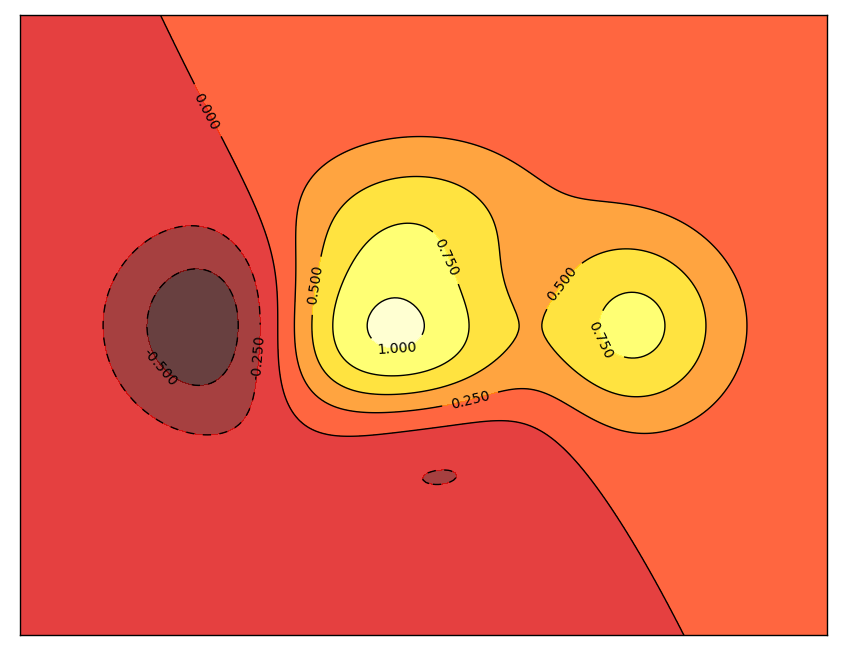
\includegraphics[width=\textwidth]{images/contour.png}
                \caption{Contour plot}                
        \end{subfigure}%        
        \begin{subfigure}[b]{0.5\textwidth}
                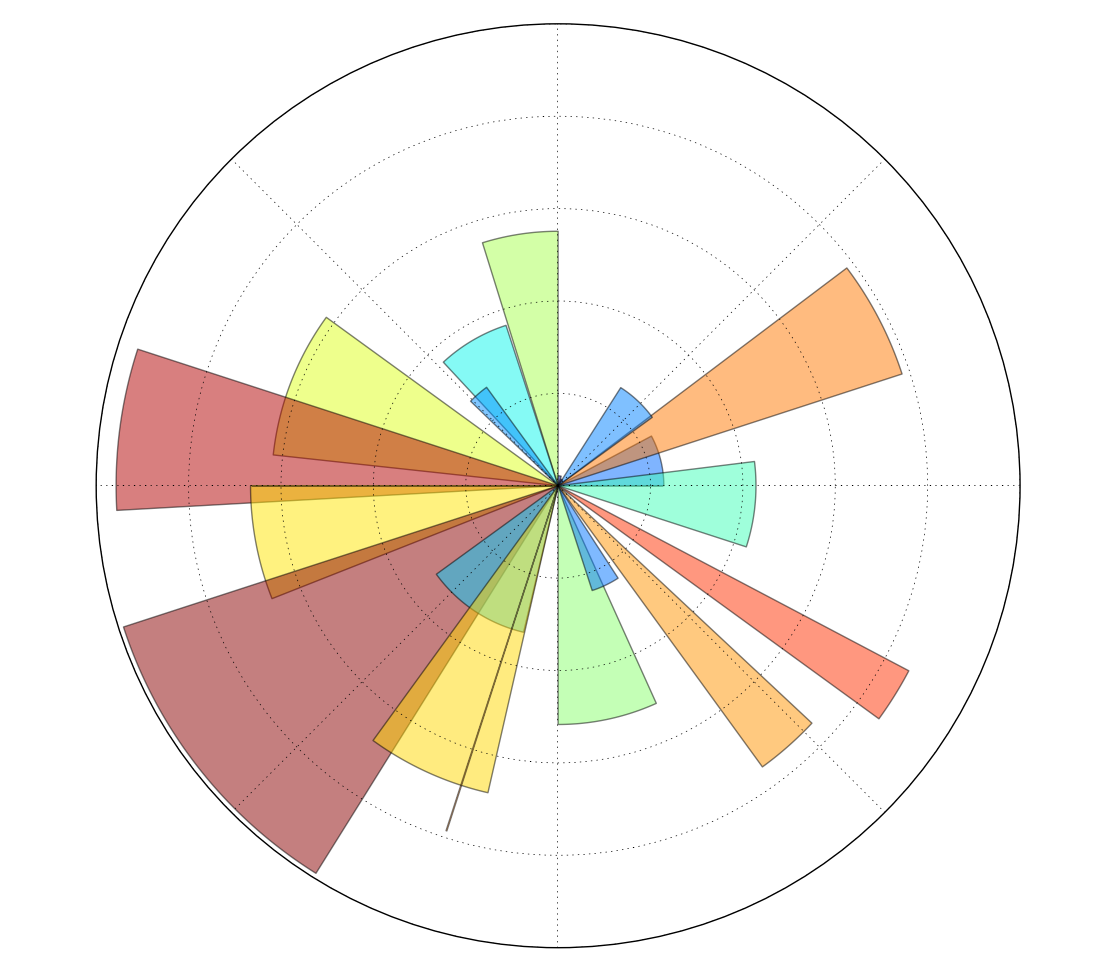
\includegraphics[width=0.9\textwidth]{images/polar.png}
                \caption{Polar plot}                
        \end{subfigure}       
        \caption{Графики, иллюстрирующие иллюстрируемое}
\end{figure}

\end{frame}

\begin{frame}[plain]
\begin{center}
{\Large Вопросы}
\end{center}
\end{frame}

\end{document}